\documentclass[11pt,a4paper, uplatex]{jsarticle}
%
\usepackage{amsmath,amssymb}
\usepackage{bm}
\usepackage[dvipdfmx]{graphicx}
\usepackage{ascmac}
\usepackage{listings}
\usepackage{underscore}
\lstset{
    frame=single,
    numbers=left,
    tabsize=2
}
%
\setlength{\textwidth}{\fullwidth}
\setlength{\textheight}{40\baselineskip}
\addtolength{\textheight}{\topskip}
\setlength{\voffset}{-0.2in}
\setlength{\topmargin}{0pt}
\setlength{\headheight}{0pt}
\setlength{\headsep}{0pt}
%
\newcommand{\divergence}{\mathrm{div}\,}  %ダイバージェンス
\newcommand{\grad}{\mathrm{grad}\,}  %グラディエント
\newcommand{\rot}{\mathrm{rot}\,}  %ローテーション
%
\title{OS 第1回課題レポート}
\author{1510151  栁 裕太}
\date{\today}
\begin{document}
\maketitle
\section{課題1: 和訳}

\subsection{OSのインターフェイス}
オペレーティングシステム(以下、OS)の仕事は、コンピュータを複数のプログラムで共有したり、
ハードウェアハードウェア単体のサポートより便利なサービスを提供することである。
そのOSは低級ハードウェアを管理・取り出しを行い、それにより、例えば、
ワードプロセッサが自身のディスクハードウェアが使用中かどうか考慮する気にする必要がなくなる。
多重のハードウェアもまた、多くのプログラムにコンピュータを同時に共有及び実行
(あるいは実行と見せかける)することを許している。
最終的に、OSは制御された相互作用する方法を提供しており、
それによってこれらはデータを共有できたり、あるいは共に仕事をすることができるのである。

単一のOSはユーザにインターフェースを介してプログラム群を提供する。
よいインターフェースをデザインすることは難しいことがわかる。
一方に、我々はインターフェースをより簡単に正しく実行するために、シンプルで精密なものにしたがる。
もう一方に、我々はより洗練された特徴をアプリケーションに提供するよう誘惑されるかもしれない。
この緊張を解くトリックは、インターフェースをもっと普遍的に提供できるようにするために、
ほんの少しメカニズムに依拠するデザインにすることである。

この本は単一のOSを実態のある例として、
OSのコンセプトを説明するために利用する。
xv6というOSは、ケン・トンプソンとデニス・リッチーによる
UNIXOSの基本的なインファーフェースを提供し、
できるだけUNIX内部のデザインを模倣したものとなっている。
UNIXはメカニズムもよく内包した限定的なインターフェースで、驚くべき汎用性を提供する。
このインターフェースはにおいて成功してきており、現代のOS
―BSD, Linux, MacOS, Solaris, そして更に、限定的では在るが、Microsoft Windowsも―
はUNIXのようなインターフェースを所持している。
xv6を理解することは、これらのシステムやその他を理解するためのよいスタート地点となるのである。

図0-1に記載されたとおり、xv6は伝統的なkernelの形式をとっており、
プログラムを走らせるためのサービスのような特別なプログラムがある。
それぞれの走っているプログラム(プロセスと呼ぶ)は、
指示/データ/スタックを内蔵したメモリを保持している。
この指示はプログラムの計算が実装されている。
データは計算における変数である。
スタックは、プログラム処理の指示が構成されてある。

プロセスがカーネルサービスを呼び出す必要がある時、まずOSのインターフェース内にて手続きを呼び出す。
この手続きのことを"システムコール"と呼ぶ。
このシステム指示がカーネル内部に入り、カーネルがサービスと結果返しを行う。
それゆえプロセスはユーザスペースとカーネルスペースとの処理のやりとりを代行しているのである。

カーネルはCPUのハードウェア保護装置を、
ユーザスペースにて各プロセス実行が自身のメモリにのみアクセスするのを確実化させるために使う。
このカーネルはこれらの保護を通過するために求められるハードウェアの権限と共に実行するため、
ユーザのプログラムらがわざわざこれらの権限を使わずに実行できる。
ユーザプログラムがシステム指示を呼び出した際に、
ハードウェアが権限のレベルと、カーネル内の既定の関数の処理実行開始を通知する。

カーネルが提供するシステム指示収集はユーザープログラムが参照するインターフェースである。
xv6のカーネルはのサービスのサブセットとUNIXカーネルがもたらすシステム指示を提供する。
その指示が以下の表の通りである。

\begin{figure}
  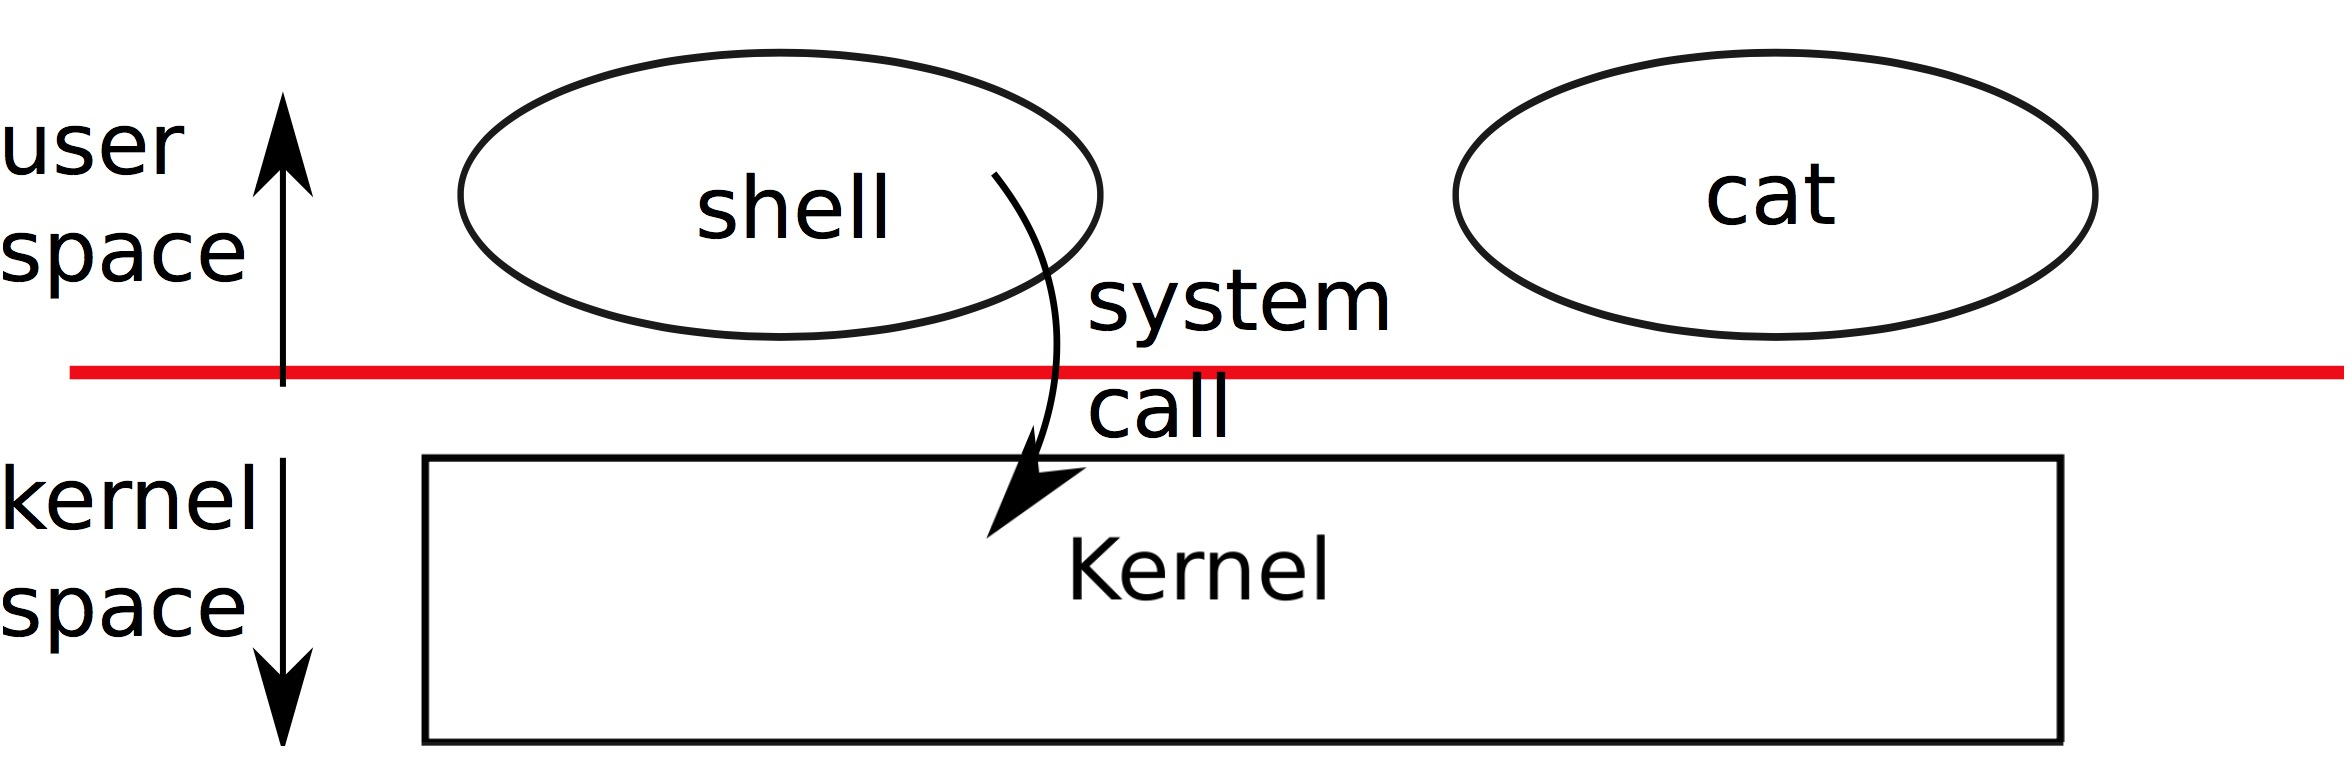
\includegraphics[width=\linewidth]{./fig1.jpg}
  \caption{1つのカーネルと2つのユーザプロセス}
  \label{fig0-1}
\end{figure}

\hrulefill

\begin{table}[htb]
  \begin{center}
    \begin{tabular}{lcrr}
      システムコール & 説明 \\
      fork() & プロセス作成 \\
      exit() & 進行中プロセスを終了 \\
      wait() & 子プロセスが終了するまで待機 \\
      kill(pid) & pid(プロセスID)のプロセスを終了 \\
      getpid() & 進行中プロセスのpidを返す \\
      sleep(n) & n秒間スリープする \\
      exec(filename, *argv) & ファイルをロードし、実行 \\
      sbrk(n) & プロセスのメモリをnバイト増やす \\
      open(filename, flags) & ファイルを開く(flagsは読込/書込を表す) \\
      read(fd, buf, n) & ファイルをbuf内へ開き、nバイト詠込む \\
      write(fd, buf, n) & ファイルを開き、nバイト詠込む \\
      close(fd) & fdにて指定した開いたファイルを閉じる \\
      dup(fd) & fdを複製する \\
      pipe(p) & パイプを開き、p内のfd群を返す \\
      chdir(dirname) & カレントディレクトリを変更する \\
      mkdir(dirname) & 新規ディレクトリ作成 \\
      mknod(name, major, minor) & デバイスファイルを作成する \\
      fstat(fd) & 開いたファイルの情報を返す \\
      link(f1, f2) & f1のファイル名をf2に変更する \\
      unlink(filename) & ファイル削除 \\
    \end{tabular}
  \end{center}
  \label{tbl1}
\end{table}

この先のチャプターにてxv6のサービス
―プロセス、メモリ、ファイル記述子、パイプ、そしてファイルシステム―
そしてこれらについてコードやスニペット、
そしてシェルがいかにこれらを使役するかという議論を用いて説明する。
そのシェルがシステムコールを使役する方法を見ることで、
いかに彼らが注意深くデザインされているのか物語ってくれるだろう。

シェルはユーザからや、実行されたものからのプログラムを読む一般的なプログラムで、
そして伝統的なUNIX的システムにおける最初のユーザインターフェースである。
シェルはユーザプログラムという事実があり、カーネルの一部ではなく、
システムコールインターフェースの力を表す例であり、すなわち
シェルにおいては特異な要素はないのである。
これはシェルは簡単に結果のような他のものに置き換えることができることもまた意味しており、
また現代のUNIXシステムは1種の選択するシェルを保持しており、
それぞれが自身のユーザインターフェースとスクリプトの特徴を併せ持っている。
xv6のシェルはUNIXボーンシェルの本質の単純なインプリメンテーションである。
このインプリメンテーションは7850行目にて説明がある。

\subsection{プロセスとメモリ}
xv6のプロセスはユーザスペースのメモリ(指示、データ、そしてスタック)と、
毎プロセスのカーネルへの内部状態を含んでいる。
xv6ははタイムシェアリングを提供し、
これが実行待ちのプロセス下におけるセット内の使用可能なCPUに判別しやすく切り替えることができる。
プロセスが実行されていないときにxv6はCPUレジスタを保持し、
次にプロセスが実行されるときにそれらを戻す。
カーネルはプロセス識別子あるいは"pid"と、それぞれのプロセスを結びつけている。

プロセスは"fork"というシステムコールで新たなプロセスを作る時がある。
forkは新たなプロセスを作り、それは子プロセスと呼ばれ、
呼び出されるメモリは全く同一のものとなり、呼び出し元のプロセスを親プロセスと呼ぶ。
forkは親子両方共を返す。
親では、forkは子のpidを、子では0を返す。
例えば、以下のプログラム片を考える。
\begin{lstlisting}[language=c]
  int pid;
  pid = fork();
  if(pid > 0){
    printf("parent: child=%d\n", pid);
    pid = wait();
    printf("child %d is done\n", pid);
  } else if(pid == 0){
    printf("child: exiting\n");
    exit();
  } else {
    printf("fork error\n");
  }
\end{lstlisting}
このexitシステムコールは呼び出したプロセスを実行停止させ、
メモリや開いたファイルなどといったリソース放棄を引き起こす。
このwaitシステムコールは現プロセスの終了した子プロセスのpidを返し、
もし対象プロセスの終了した子がない場合は、waitでは終了するまで待機する。
例えば、これらの出力では
\begin{lstlisting}
  parent: child=1234
  child: exiting
\end{lstlisting}
はもしかしたら順番が前後しているかもしれなく、
これは親あるいは子のどちらが先にprintfコールを得たかに依存する。
子が終了し親のwaitシステムコールの返り値を得ることで、
親が以下を出力する
\begin{lstlisting}
  parent: child 1234 is done
\end{lstlisting}
親と子はそれぞれ異なるメモリとレジスタで実行されていることに注意しなければならず、
1つの変数を変更することが他所へ影響を及ぼすことはない。

このexecシステムコールは呼び出したプロセスのメモリを、
新たなファイルシステムに所蔵されたファイルから読み込んだメモリイメージ移動させる。
このファイルは必ず特定のフォーマットを保持していなければならず、
また内部には指示、データ部分、何処から指示が始まるか、等を指定ファイルに明記する必要があり、
xv6はELFフォーマットを使用しており、詳細はChapter2にて記されている。
execが成功した時、何も呼び出したプログラムには値を返さず、そのかわりに
ELFヘッダ内にて、実行ファイルから読み込み、明示された開始ポイントを返す。
execは2つの引数があり、実行可能なファイルの名前と文字列を渡す。以下に例を示す。
\begin{lstlisting}
  char *argv[3];
  argv[0] = "echo";
  argv[1] = "hello";
  argv[2] = 0;
  exec("/bin/echo", argv);
  printf("exec error\n");
\end{lstlisting}
このフラグメントは呼び出したプログラムを、引数の一覧である"echo hello"を
ある/bin/echoのプログラムのインスタンスへ送っている。
多数のプログラムは最初の引数を無視しており、旧来のプログラムの名前として扱っている。

このxv6のシェルは上位の呼び出しをユーザに変わってプログラムを走らせている。
メインのシェルの構造は単純で、main(8001)を参照のこと。
メインのループはコマンドライン上で"getcmd"によって入力を読み込んでいる。
それからforkと呼ばれ、シェルの往路セスのコピーを作成する。
親のシェルはwaitと呼ばれるコールで、しばらく子プロセスがコマンドを走らせる。
例えば、もしユーザが"echo hello"とプロンプトで打った場合、
runcmdは"echo hello"を引数として呼び出すことになるだろう。
runcmd(7906)は実際のコマンドを走らせる。
"echo hello"に関しては、こちらはexec(7926)を呼び出すだろう。
もしexecが完了したらその後は子供はruncmdの代わりにechoによる指示を実行するだろう。
いくつかの点においてechoはexitを呼び出し、
これが親にmain(8001)におけるwaitの値を返すのを引き起こすだろう。
あなたはどうしてforkとexecが別々ではなく、単独の呼び出しに統一されないのか気にするかもしれないが、
我々はこのあとプロセス作成とプログラム読み込みが別々であることが、
クレバーなデザインであることを知ることになるだろう。

xv6は多くののユーザスペースのメモリを暗に割り当てており、例えば
forkはメモリを親のメモリから子へコピーするために求められるだけ割り当てており、
そしてexecは実行できるファイルを保有するために必要なメモリを割り当てる。
1つのプロセスはあるときにより多くのメモリを要す。なぜならば
ランタイム(おそらくは、mallocのため)が、
sbrk(n)を呼び出してメモリをnバイト増やし、
sbrkが新規メモリの位置を返せられるようにする必要があるからである。

xv6はユーザを他所から来たユーザから守るという概念は提供しておらず、
UNIXの部分においては、すべてのxv6のプロセスはrootとして処理が行われる。
%
%
\end{document}
